\documentclass{article}

\usepackage[utf8x]{inputenc}
\usepackage{hyperref}
\usepackage[ngerman]{babel}
\usepackage{url}
\usepackage{graphicx}
\usepackage{xcolor}
\usepackage{listings}
\usepackage{ulem}
\usepackage{float}
\usepackage{subfig}
\usepackage{textpos}
\usepackage{amsfonts}
\usepackage{amsmath}
\usepackage[bottom]{footmisc}
\newcommand{\Mod}[1]{\ (\mathrm{mod}\ #1)}

\lstset{
	basicstyle=\scriptsize\ttfamily,
	numbers=left,
	frame=single,
	breaklines=true,
	breakautoindent=true,
	postbreak={\mbox{$\hookrightarrow$}},
	literate={ä}{{\"a}}1 {ö}{{\"o}}1 {ü}{{\"u}}1 {ß}{{\ss}}1 {Ä}{{\"A}}1 {Ö}{{\"O}}1 {Ü}{{\"U}}1}

\hypersetup{
    colorlinks=false,
    pdfborder={0 0 0},
}

\renewcommand{\ttdefault}{pcr}
\DeclareOldFontCommand{\tt}{\normalfont\ttfamily}{\mathtt}



\setlength{\topmargin}{1.5cm}
\setlength{\headheight}{12pt}
\setlength{\headsep}{20pt}
\setlength{\topskip}{12pt}
\setlength{\evensidemargin}{0pt}
\setlength{\oddsidemargin}{10mm}
\setlength{\textheight}{230mm}
\setlength{\textwidth}{150mm}
\setlength{\voffset}{-2cm}
\setlength{\parindent}{0pt}
\setlength{\parskip}{6pt}

\title{
%
\includegraphics[height=2cm]{../Vorlage/hgi_nds_1.png}\\\vspace{1cm}
Angriffe auf RSA\\\vspace{7mm}
Grundlagenpraktikum zur IT-Sicherheit\\(WiSe 2019/2020)\\\vspace{1cm}
\large{Horst Görtz Institut für IT-Sicherheit\\
Ruhr-Universität Bochum
\\\vspace{1cm}}}

\begin{document}

\maketitle
\thispagestyle{empty}

\begin{abstract}
\noindent
In diesem Kapitil beschäftigen wir uns mit Angriffen auf RSA, dabei gehen wir nicht auf mathematische Angriffe ein, sondern analysieren, was in der Praxis falsch laufen kann. Im ersten Schritt wird RSA falsch verwendet, im zweiten und dritten Schritt machen wir es uns zu nutzte, dass die CPU unter bestimmten Bedingungen falsch rechnet und so ein falsches Ergebnis liefert, welches wir für den Angriff nutzen können.
\end{abstract}
\newpage
\thispagestyle{empty}
\tableofcontents

\newpage
\setlength{\parindent}{0pt}
\setcounter{page}{1}
\section{Einleitung}
RSA ist in der Praxis immernoch ein weit verbreitetes asymmetrisches Verschlüsselungsverfahren, welches in viele Anwendungen wie zum Beispiel PGP, TLS und SSH zum Einsatz kommt, um nur einige von ihnen zu nennen. Zwar wird elliptische Kurven Kryptographie immer beliebter, da es nicht so große Schlüssel braucht, jedoch wird dieses Verfahren im Quantencomputer Zeitalter als erstes Fallen, da es die kleinsten Schlüssel hat. RSA ist das erste asymmetrische kryptographische Verfahren, dass der Öffentlichkeit bekannt wurde, was das Militär und die Geheimdienste im verschlossenen so benutzten, ist ja nicht öffentlich. Der Name RSA leitet sich von den Entwicklern ab, Rivest Shamir und Adleman. Da RSA auf dem mathematischen Problem der Primfaktorzerlegung beruht, ist es nur so lange sicher, solange niemand diese Problem gelöst hat. Dieses besagt, dass es äußerst schwer ist eine Zahl n in ihre Primfaktoren zu zerlegen aber es sehr leicht ist, mehreren Primfaktoren zu multiplizieren. So eine Konstruktion wird auch Trapdoorfunction oder Einwegfunktion genannt. Neben den mathematischen Angriffen, von denen der Index-Calculus der mächtigste ist, gibt es auch eine Reihe praktische Probleme und Fehler, die bei der Verwendung von RSA auftauchen. Diesen Problemen widmen wir uns in diesem Versuch, da eine detaillierte Analyse aller Angriffe den Bogen überspannen würde, schauen wir uns hier nur einige Angriffe an.
\subsection{Glossar}
%\begin{description}
%\end{description}
\newpage % jede section sollte auf einer neuen Seite starten
\section{Aufbau}
In diesem Versuch arbeiten wir wieder an den Computern im Netzlabor. Es kommt ebenfalls wieder Ubuntu-Mate zum Einsatz. Entgegen der Versuchsbeschreibung nutzen wir Ubununtu 14.10 als Basis nicht Ubuntu 10.04. Uns wurden verschiendene Webapplikationen zur Verfügung gestellt. Uns steht unter \href{http://192.168.2.6/smartcard}{http://192.168.2.6/smartcard} die Möglichkeit zur Verfügung, Zahlen signieren zu lassen und gegebenenfalls einen Fehler bei der Rechnung zu veranlassen. Unter \href{http://192.168.1.6/bugattack}{http://192.168.1.6/bugattack} ist eine ähnliche Anwendung, aber ohne die Möglichkeit einen Fehler per klick selbst zu initiieren. Hier entsteht ein Fehler bei bestimmten Zahlen als Eingabeparameter.
\begin{figure}[H]
  \centering
  \subfloat[][]{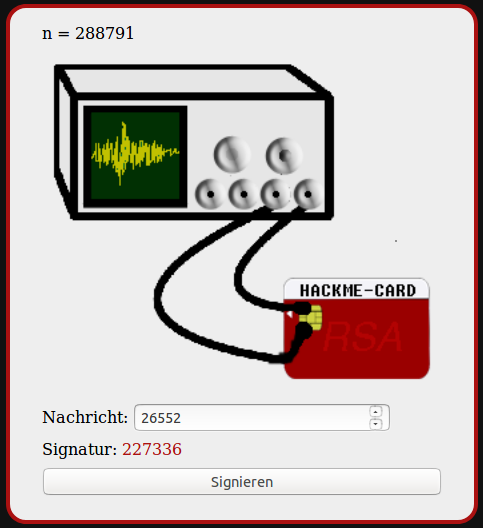
\includegraphics[width=0.4\textwidth]{../Aufbau_1.png} }
  \qquad
  \subfloat[][]{\includegraphics[width=0.4\textwidth]{../Aufbau_2.png} }
  \caption{Webapplikationen}
  \label{fig:1}
\end{figure}
\newpage % jede section sollte auf einer neuen Seite starten
\section{RSA-Verschlüsselung mit kleinem öffentlichen Exponenten}
In dieser Aufgabe war es Ziel, mehrere RSA-Signaturen kleinem öffentlichen Exponenten anzugreifen. Zuerst mussten wir an die Parameter kommen. Diese lagen als Datei im PEM Format vor. Der OpenSSL Befehl um die kryptographischen Parameter zu extrahieren ist in Listing \ref{lst:1} zu sehen.
\begin{lstlisting}[caption={OpenSSH Befehl für RSA Parameter aus PEM Datei},captionpos=b,float=ht!,label=lst:1]
student@Reihe2-PC5:~/Praktikum/rsa$ openssl rsa -in "DATEI".pk -noout -pubin -modulus -text
\end{lstlisting}
\\Die öffentlichen Schlüssel sind in allen drei Fällen drei und die Module sind bei Costa $3748150753$, bei Gambino $3012222769$ und bei Zarella $3715158301$. Es waren nun 3 Chiffrate gegeben, die den gleichen Klartext verschlüsseln. Jedoch unterschiedliche private Schlüssele und Module verwenden. Nun war es die Aufgabe den Klartext herauszufinden. Dabei nutzen wir den chinesischen Restsatz. Anstatt alles mühselig im Taschenrechner zu rechnen, haben wir ein Script geschrieben, mit dem sich die Kongruenzen lösen lassen. Dieses ist in Listing \ref{lst:2} zu sehen.
\begin{lstlisting}[caption={Script zum lösen dreier linearer Kongruenzen},captionpos=b,float=ht!,label=lst:2]
import math
import gmpy2
c = [0xdf683de1,1786058302]
z = [0xb38adf31,521332323]
v = [0xdd70d11d,2806221682]

g_m = c[0]*z[0]*v[0]

m1 = z[0]*v[0]
m2 = c[0]*v[0]
m3 = z[0]*c[0]

inv_m1 = gmpy2.invert(gmpy2.mpz(m1%c[0]),c[0])
inv_m2 = gmpy2.invert(gmpy2.mpz(m2%z[0]),z[0])
inv_m3 = gmpy2.invert(gmpy2.mpz(m3%v[0]),v[0])

inv_m1 = int(inv_m1.digits(),10)
inv_m2 = int(inv_m2.digits(),10)
inv_m3 = int(inv_m3.digits(),10)

m_hoch_3 = (c[1]*inv_m1*m1%g_m + z[1]*inv_m2*m2%g_m + v[1]*inv_m3*m3%g_m)%g_m
print(m_hoch_3)
m = math.pow(m_hoch_3,1/3)
m = math.ceil(m)
m = "0"+str(m)
print(m)
\end{lstlisting}
\\In Zeile drei bis 5 werden die bekannten Werte in ein Array geschrieben. Wir wollen drei Kongruenzen gleichzeitig lösen. \\
\begin{align}
1786058302 \equiv x \mod 3748150753 \\
521332323  \equiv x \mod 3012222769 \\
2806221682 \equiv x \mod 3715158301 
\end{align}
Nach dem Satz müssen wir zunächst M berechnen, welches der Multiplikation aller Module entspricht. Dann müssen die $M_i$'s bestimmt werden, welche sich durch $\frac{M}{m_i}$ berechnen, wobei $m_i$ den Modulus der i-ten Gleichung entspricht. Dies geschieht in Zeile dreizehn bis fünfzehn. Im nächsten Schritt müssen wir die Multiplikative Inverse von $M_i \mod{m_i}$ bestimmen. Nachdem wir dies für alle \textit{i} getan haben müssen wir das Endergebnis nur noch aus den Gleichungen zusammensetzen. Dies tun wir in Zeile 21. Dabei nehmen wir die bekannten Lösungen der Gleichungen, $y_i$ multiplizieren sie mit $M_i$ und der Inversen von $M_i$ und reduzieren Modulo $M$. Dies tun wir für alle \textit{i} addieren die Ergebnisse auf und rechnen das Endergebnis erneut Modulo $M$.
Heraus bekommen wir die Nachricht $x^3$. Nun ziehen wir noch die 3 Wurzel und bekommen als Ergebnis mit führender Null $084114101$ heraus. Nun nutzen wir die Pythonfunktion \textbf{chr()}, um die Blöcke zu konvertieren. Als Lösungswort bekommen wir \textbf{Tre} heraus, was auf Deutsch drei bedeutet
\newpage
\section{Fault-Angriff gegen RSA-CRT}
In diesem Schritt nutzen wir eine, der bereits im Aufbau beschriebenen, Webapplikationen für den Versuch. Konkret sollen wir mittels Fault-Angriff $n=p \cdot q$ faktorisieren. Zur Verfügung steht uns hierbei der Webapplikatione, die richtig berechnete Signaturen ausgeben kann, oder sich verrechnet und dann falsche Werte ausgibt. Allgemein berechnet sich die Signatur über den chinesischen Restatz mit $s = (q^{-1}\mod{p}) \cdot m_p^{d_p}\cdot q + (p^{-1}\mod{q}) \cdot m_q^{d_q}\cdot p$. Ersetzt man nun $(q^{-1}\mod{p})\cdot m_p^{d_p}$ durch X, so ergibt sich $s = X\cdot q + (p^{-1}\mod{q}) \cdot m_q^{d_q}\cdot p$ .\\
Haben wir nun 2 Signaturen gegeben, eine gültige und eine, in der ein Teil falsch gerechnet wurde, können wir die gefälschte Signatur von der Originalen abziehen, dabei ist es egal ob der vordere oder der hintere Teil einen Fehler aufweist. Wichtig ist nur, das ein Teil korrekt berechnet wurde. Wir gehen im nachfolgenden davon aus, dass $(q^{-1}\mod{p})\cdot m_p^{d_p}$ falsch berechnet wurde. Diesen Wert ersetzen wir durch X.
\begin{align}
&s = (q^{-1}\mod{p}) \cdot m_p^{d_p}\cdot q &+ (p^{-1}\mod{q}) \cdot m_q^{d_q}\cdot p \\
&s' = X\cdot q &+ (p^{-1}\mod{q}) \cdot m_q^{d_q}\cdot p \\
&s-s' = ((q^{-1}\mod{p}) \cdot m_p^{d_p}-X)\cdot q \\
&s-s' = Y \cdot q 
\end{align}
Berechnen wir nun den ggt von $s-s'$ und n, so bekommen wir die erste Zahl der Primfaktorzerlegung heraus. Nun müssen wir n durch diese Zahl teilen und bekommen die jeweils andere. Wir haben n nun faktorisiert. Wir haben eine gültige Signatur für die Zahl 10 erstellt. s wurde signiert mit dem Wert 158338. Nun haben wir vier falsche Signaturen erzeugt, 7, 100224, 154187 und 155373. Es wurde erneut die Pythonkonsole genutzt und die mathematische Funktion \textit{math.gcd()}, was für \textbf{G}reatest \textbf{C}ommon \textbf{D}ivisor steht. Es kam vier Mal die Zahl 593 heraus, welche p entspricht. n geteilt durch p war 487, was q entspricht. Die Primfaktorzerlegung war erfolgreich. Nun können wir d,e und $\varphi(n)$ berechnen und nach belieben Signaturen für selbst erstellte Nachrichten erzeugen.
\newpage
\section{Bug-Attack}
Die letzte Aufgabe dieses Versuchs ähnelt der vorherigen. So werden wir einen Fehler in der Berechnung, dieses mal nicht durch Fremdeinwirkung, wie Hitze oder Spannungsglitsches hervorrufen, sondern durch geschickte Wahl der zu signierenden Zahl. Manche Prozessoren rechnen bei manchen Zahlen am Eingang zu einer bestimmten Wahrscheinlichkeit falsch. Dies machen wir uns in diesem Angriff zu nutze, um die eine gültige und eine ungültige Signatur zu erzeugen. Da die Webapplikation jedoch so gut wie immer falsch rechnet nutzen wir hier 2 falsche Signaturen. Dies ändert am Angriff wenig, da sich der Prozessor nur auf 'einer Seite' verrechnet.\\
n ist in unserem Fall 207703 und der öffentliche Schlüssel $e = 17$. Die Aufgabe war es nun ein geeignetes m zu finden, eines das $\mod{p}$ reduziert wird und $\mod{q}$ nicht reduziert wird. Wir ziehen die zweite Wurzel aus n und bekommen so eine Zahl heraus, die dies erfüllt, $207703^{\frac{1}{2}}=455.744$. Diese Zahl löst jedoch keine Fehler bei der Berechnung aus. Die letzten beiden Hexadezimalziffern müssen 0x4 und 0xb entsprechen. Dies entsprich in Binärdarstellung $00101011_2$ beziehungsweise $10110010_2$. Wir haben uns dafür entschieden die Zahl $1100101011_2$ zu nehmen, was 843 entspricht.
\begin{figure}[H]
\centering
\includegraphics[width=0.7\textwidth]{../3_2.png}
\caption{Webapplikation Bug-Attack}
\label{fig:2}
\end{figure}
Wir haben zwei falsche Signaturen generiert, diese voneinander abgezogen, und den ggt von dem Ergebnis mit n berechnet. Als Ergebnis der faktorisierung bekamen wir $p = 229 \;\;\; q = 907$. Alternativ kann es wie in der Versuchsbeschreibung berechnet werden. 
\begin{align}
math.gcd(154318^{17}-843,207703) = 229
\end{align}
\newpage
\section{Zusammenfassung und Fazit}
Im neunten Versuch dieses Grundlagenpraktikums ging es um Angriffe gegen RSA und der damit zusammenhängenden Thematik praktische Sicherheit von Kryptographie. Um uns eine Einführung in dieses Thema zu geben sollten wir verschiedene Aufgaben bearbeiten.\\
Zu allererst ging es um Angriffe gegen zu kleine Exponenten im RSA Verfahren und der Ausnutzung dieser mit dem chinesischen Restsatz. Diese Aufgabe war sehr interessant, da Sie ebenfalls den Bezug zu anderen Veranstaltungen an der Uni gezogen hat. So konnten wir unser Wissen aus diskrete Mathematik einbrigen, um diese Aufgabe zu lösen.
Die zweite und dritte Aufgabe, haben gezeigt, dass man kryptographie nicht nur auf Software und mathematischer Ebene angreifen kann, sondern auch die Hardware. So nutzten wir Fehler in dieser, um an die kryptographischen Schlüssel beziehungsweise in unsere Fall zu allerst an die Primfaktorzerlegung der Zahl zu kommen.
Der Versuch hat uns einen schönen kurzen Einblick in die Thematik rund um Angriffe gegen RSA gegeben. Der Versuch hatte in der Kürze dennoch Würze und hat uns daher eine Menge Spaß bereitet. Wir freuen uns auf den nächsten Versuch. \\ 
\newpage
%
% ---- Bibliography ----
%
\end{document}
